% !TeX spellcheck = it_IT
\section{Cos'è la realtà virtuale?}

La realtà virtuale (VR) è in costante evoluzione, rendendo difficile darne una definizione specifica che non decada nel giro di pochi anni. Il modo migliore per descriverla è quindi considerare gli aspetti intrinseci cruciali che prescindono la tecnologia utilizzata.La sua concezione deve essere abbastanza generale da abbracciare sia la realtà virtuale dei nostri giorni sia quella che verrà in futuro.
\subsection{Definizione della realtà virtuale}

\begin{quotation}"Indurre un comportamento premeditato attraverso l'uso di stimolazioni sensoriali artificiali in un organismo che ha una minima, se non nulla, consapevolezza dell'interferenza."\cite{VRbook}
\end{quotation}	
In questa possibile definizione di realtà virtuale compaiono quattro componenti chiave:

\begin{enumerate}
	\item \textit{Comportamento premeditato:} l'organismo sta facendo un' esperienza designata dal creatore
	che non coincide con la cognizione del mondo reale.
	\item \textit{Organismo:} si utilizza la parola organismo poiché qualsiasi essere vivente può immergersi in un ambiente virtuale. I neurobiologi dell'Università di Monaco effettuarono i primi test sperimentali sulla VR sottoponendo dei topi da laboratorio a stimoli visivi mentre correvano su un tapis roulant sferico. Altri esperimenti sono stati fatti su scimmie, pesci, scarafaggi e moscerini.
	\item \textit{Stimolazioni sensoriali artificiali:} attraverso degli strumenti tecnologici uno o più sensi dell'organismo vengono deviati e i loro input ordinari sono sostituiti da quelli artificiali
	\item \textit{Consapevolezza:} durante l'esperienza virtuale l'organismo viene "ingannato" nel sentirsi presente in un mondo fittizio e non essendone conscio lo accetta come naturale.
\end{enumerate}

\begin{wrapfigure}{r}{0.35\textwidth} %this figure will be at the right
	\centering
	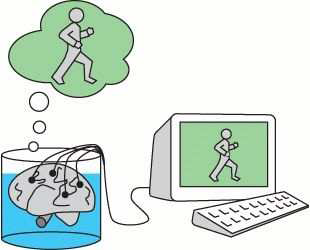
\includegraphics[width=0.25\textwidth]{figure/VRfool}
\end{wrapfigure}
Quest'ultimo fattore può sembrare frivolo, ma ci offre un'ulteriore possibilità di vedere in cosa consiste concretamente la realtà virtuale. Numerosi ricercatori di neurobiologia hanno dimostrato che il cervello di un animale sottoposto ad un'esperienza virtuale \mbox{genera} strutture cerebrali formate da \textit{cellule di posizione e cellule grid}, contenenti le informazioni spaziali dell'ambiente circostante, proprio come accade nell'esplorazione di luoghi reali.\\
Un'altra componente cruciale della realtà virtuale è l'\textit{interazione}: se la stimolazione sensoriale non dipende dalle azioni compiute dall'utente, il sistema VR viene definito \textit{open-loop} ed è il più semplice grado di virtualizzazione della realtà. In caso contrario la configurazione viene chiamata \textit{closed-loop}. In quest'ultima l'organismo ha un controllo parziale sulla manipolazione sensoriale, che potrebbe variare a seconda dei movimenti del corpo (testa,braccia,gambe,occhi,etc.), di comandi vocali, frequenza cardiaca, temperatura del corpo, resistenza elettrica cutanea (sudore).\\ E' infatti consuetudine far combaciare il più possibile la simulazione con il mondo fisico riproducendone anche le interazioni,poiché essendo il nostro cervello più familiare con queste, accetterà più facilmente l'ambiente come naturale.
\newpage

\subsection{Lo stato dell'arte}

Siamo entrati nell'età moderna della realtà virtuale grazie agli avanzamenti nelle tecnologie di visualizzazione, percezione e computazionali portate dall'industria degli smartphones. I visori di realtà virtuale ora vengono prodotti in massa e distribuiti ad un'ampia varietà di persone. Questa tendenza è molto simile alle rivoluzioni da cui nacquero i personal computer e i web browser: maggiore è il numero di persone che hanno accesso alle tecnologie, maggiori sono le possibilità di queste ultime.
\subsubsection{Applicazioni }
Al giorno d'oggi la VR è attiva nei seguenti campi \cite{VRApplications}:
\begin{enumerate}
	\item \textit{Videogiochi:} forse il campo in cui ha raggiunto la sua massima espressione ed il settore che traina la distribuzione su larga scala dei visori per la realtà virtuale.
	\item \textit{Militare:} ampiamente adottata dagli eserciti di molte nazioni per l'addestramento delle proprie truppe, poiché permette loro di imparare come reagire in situazioni ostili evitando i rischi e i costi delle vecchie simulazioni e aumentando il grado di realismo nello stress provato dai soldati (simulatori di combattimento,medicina da campo, guida di veicoli militari,etc.).
	\item \textit{Medicina:} spesso utilizzata per la simulazione di interventi chirurgici, superamento interattivo di fobie, chirurgia robotica, diagnostica, trattamenti per persone portatrici di handicap e per l'insegnamento.
	\item \textit{Moda:} attraverso cataloghi virtualizzati e progettazioni di negozi allestiti precedentemente in VR.
	\item \textit{Sport:} utile per migliorare le performance degli sportivi attraverso appositi ambienti virtuali, ma anche per avvicinare il pubblico mettendolo al centro dell'evento sportivo o facendogli vedere in anteprima come sarà la visuale dal suo posto dello stadio.
	\item \textit{Visualizzazione scientifica:} per mostrare più facilmente grosse moli di dati o informazioni complesse facilitando le collaborazioni interdisciplinari.
	\item \textit{Costruzione e Design:} le esplorazioni virtuali danno la possibilità di avere un feedback più realistico delle nuove strutture o soluzioni di design, come organizzazione di interni o progettazione di nuovi prodotti, prima ancora di realizzarli.
	\item \textit{Istruzione:} rende più diretto l'apprendimento in molte discipline che sarebbero difficili da visualizzare o ricordare, soprattutto nella scuola dell'infanzia.
	\item \textit{Media e informazione:} con l'utilizzo di film e documentari interattivi o di report giornalistici in cui l'utente è al centro della notizia e la può vivere in prima persona
	
\end{enumerate}
\vspace{0.4cm}
\subsubsection{Hardware}

Il primo passo per capire come funziona la realtà virtuale è considerare cosa costituisce un intero sistema VR.
Al contrario di quanto si possa pensare, non si tratta solamente delle componenti fisiche, come il visore, il computer o i controllers, ma l'organismo utilizzatore è altrettanto fondamentale. Per facilità in questo capitolo verrà considerato un essere umano .\\
il cervello decodifica lo spazio fisico, sia reale che virtuale, mediante la ricezione di input sensoriali. E' in grado di controllare la configurazione di questi ultimi mentre ne riceve le informazioni, permettendo la creazione di coordinate "coscienti" dello spazio circostante l'individuo.\\
\begin{figure}[H]
	\centering
	\begin{minipage}[b]{0.49\textwidth}
		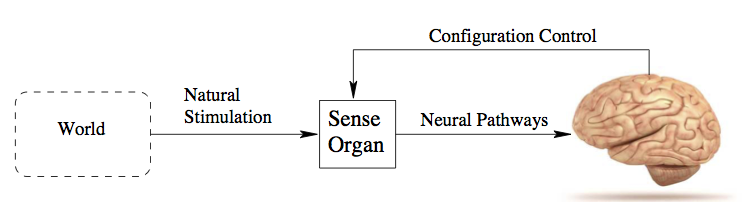
\includegraphics[width=\textwidth]{figure/RealityBB}
		{\footnotesize \centerline{(a)} \par}
	\end{minipage}
	\hfill
	\begin{minipage}[b]{0.49\textwidth}
		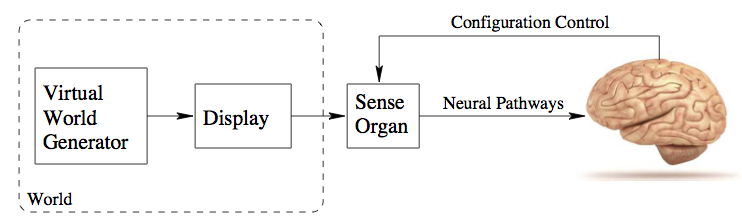
\includegraphics[width=\textwidth]{figure/VRBB}
			{\footnotesize \centerline{(b)} \par}
	\end{minipage}
	\caption{Il processo di raccolta, analisi e controllo di informazioni sensoriali nel mondo reale (a) e in quello virtuale(b).}
\end{figure}

\newpage

L'hardware di una configurazione in realtà virtuale deve tenere traccia dei movimenti dell'utente per regolare gli stimoli artificiali in modo corretto, dando il desiderato senso di immersione.
Un fattore di fondamentale importanza è lo studio degli spostamenti della testa nello spazio, in quanto codificati dal sistema nervoso centrale come un insieme di stimoli visivi, uditivi e vestibolari. \\
Per aumentare il grado di realismo della simulazione si tende a monitorare i movimenti di braccia o gambe. Infine è in egual modo significativo prendere in considerazione l'ambiente reale circostante come parte integrante del sistema VR perché, nonostante  le stimolazioni controllate, l'utilizzatore  continuerà a percepirlo.
\begin{figure}[H]
	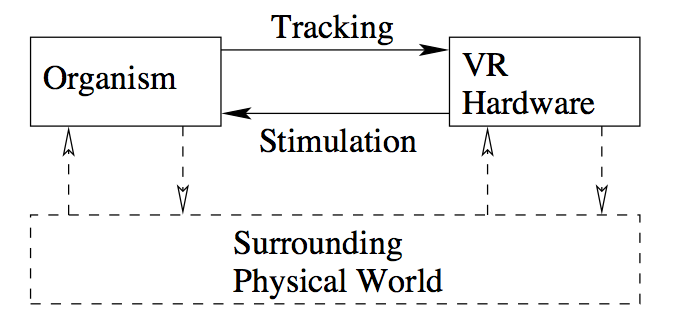
\includegraphics[width=0.65\textwidth]{figure/TrackingStimuliBB}
	\centering
	\caption{Lo schema di un sistema VR}
\end{figure}

\newpage

Scendendo più nei dettagli i moderni sistemi di VR sono composti da tre componenti hardware principali: display, sensori, computer.
\begin{flushleft}
	\underline{\textit{Displays}:}
\end{flushleft}  Attraverso di essi avviene la stimolazione degli organi sensoriali, in particolare della vista e dell'udito.. Nei sistemi {CAVE}, un acronimo ricorsivo che sta per "cave automatic virtual enviroment", l'utente è avvolto da immagini 3D proiettate su sei piani di visualizzazione fissi ed immerso in un'audio sorround. Nei sistemi \textit{HMD}, head-mounted display, la configurazione consiste, come da definizione, in un visore montato sulla testa. Nei modelli più semplici viene utilizzato lo schermo di un cellulare e due lenti focali per gli occhi come nel caso dei Google Cardboard. Le apparecchiature più sofisticate utilizzano schermi progettati appositamente per la VR, che sfruttano la tecnologia LED 
o strumenti di \textit{proiezione pico}, come \textit{DLP(Digital Light Processing), LCD(Liquid Crystal Display)} o \textit{LQoS(Liquid Crystal on Silicon)}.Alcuni prodotti che implementano queste tecnologie sono \textit{ Google Glass}, \textit{Microsoft Hololen}s e \textit{Avegant Glyph}. Prototipi in fase di sviluppo sono gli schermi a \textit{campi luminosi} \cite{LFD} e a \textit{piani focali multipli} \cite{MFP}, purtroppo ancora poco competitivi perché non utilizzate nel mercato dei dispositivi mobili. 

\vspace{0.2cm}

\begin{figure}[H]
	\centering
	\begin{minipage}[b]{0.49\textwidth}
		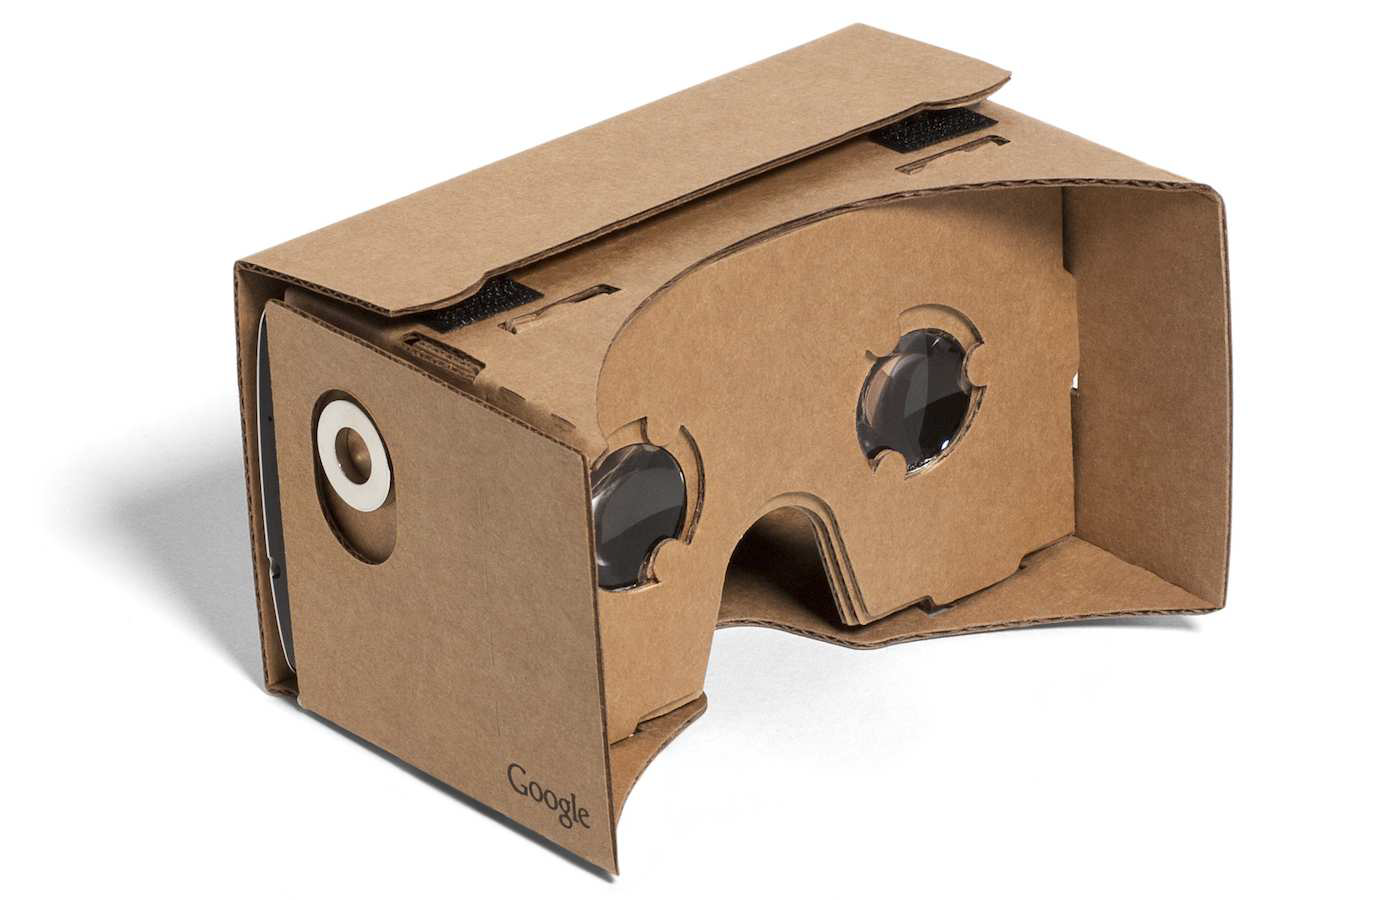
\includegraphics[width=\textwidth]{figure/Cardboard}
		{\footnotesize \centerline{(a)} \par}
	\end{minipage}
	\hfill
	\begin{minipage}[b]{0.49\textwidth}
		\includegraphics[width=\textwidth]{figure/Oculus}
		{\footnotesize \centerline{(b)} \par}
	\end{minipage}
	\caption{I Google Cardboard,un visore molto rudimentale (a) e un modello di Oculus DK2 con display integrati(b).}
\end{figure}

\newpage

\begin{flushleft}
	\underline{\textit{Sensori}:}
\end{flushleft}  Per generare il corretto output artificiale vanno costantemente monitorati gli organi di senso dell'individuo, in particolare la loro posizione e l'orientamento. Per quest'ultimo si impiega usualmente un'\textit{unità di misura interna} (IMU), formata da un giroscopio le cui misure sono integrate nel tempo dando una stima dell'inclinazione. Il rumore generato da questa misurazione, definito come errore di derivazione, può essere annullato o ridotto con l'impiego di altri strumenti come accelerometri e magnetometri.\\
A metà del secolo scorso le IMU erano pensabili solamente su velivoli e missili, dati i costi e le dimensioni molto elevate, ma al giorno d'oggi sono incorporate nel gran parte dei dispositivi mobili e sono la nuova tecnologia che ha portato ad una distribuzione su ampia scala della realtà virtuale.\\
Un'altra tecnologia che è diventata più accessibile sono le \textit{telecamere digitali} grazie alle quali si può adottare un approccio di monitoraggio \textit{visivo}.
L'idea è di identificare nell'immagine dei \textit{markers} o elementi fissi, che fungono da riferimento per il sistema. Questo processo impone però dei limiti sulla potenziale posizione o orientamento dei visori ed è per questo che sono in via di sviluppo intelligenze artificiali addette al riconoscimento di immagini che scalzino l'impiego di marker fisici.

\vspace{0.2cm}

\begin{figure}[H]
	\centering
	\begin{minipage}[b]{0.49\textwidth}
		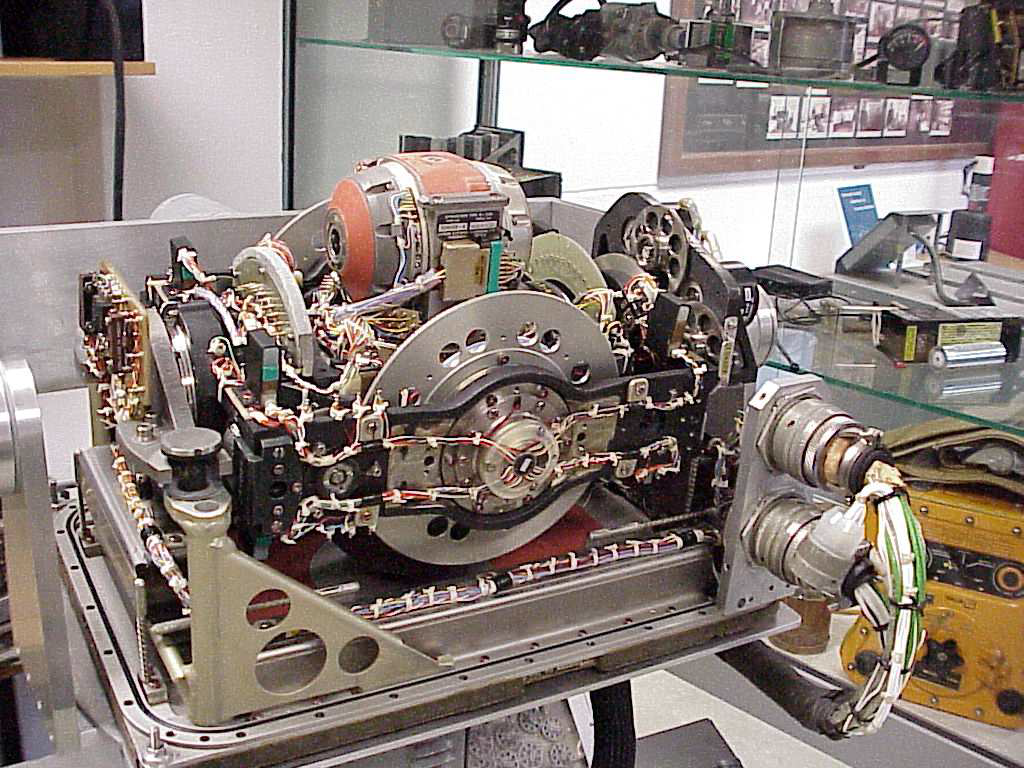
\includegraphics[width=\textwidth]{figure/oldIMU}
		{\footnotesize \centerline{(a)} \par}
	\end{minipage}
	\hfill
	\begin{minipage}[b]{0.46\textwidth}
		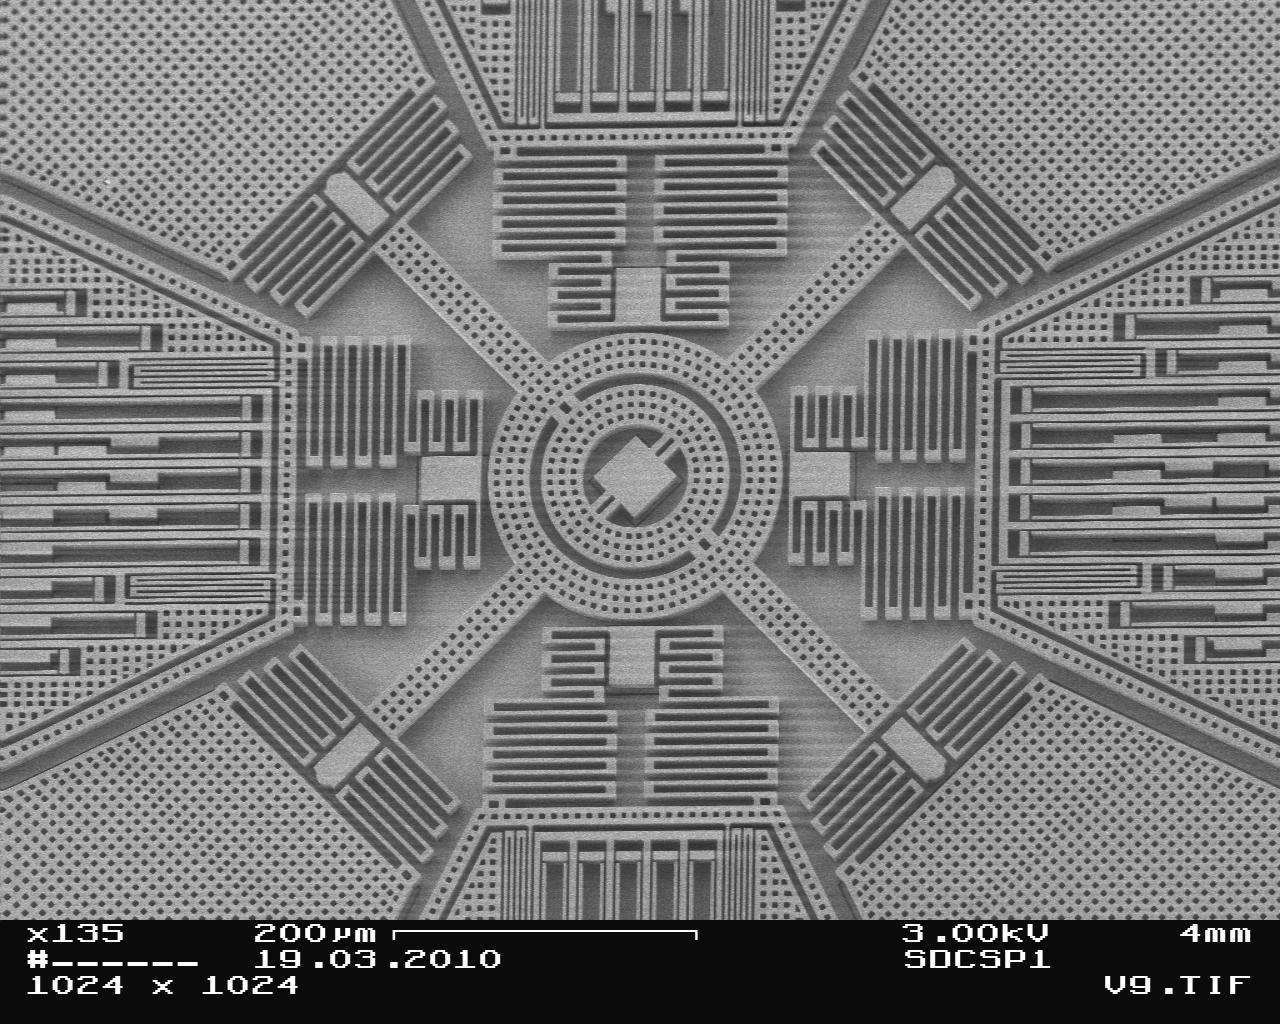
\includegraphics[width=\textwidth]{figure/IMU}
		{\footnotesize \centerline{(b)} \par}
	\end{minipage}
	\caption{Un modello di IMU (LN-3 Inertial Navigation System) sviluppato negli anni '60 dalla Litton Industries (a) e un modello odierno situato in un giroscopio MEMS largo meno di un millimetro. (b)}
\end{figure}

\newpage

\begin{flushleft}
	\underline{\textit{Computers}:}
\end{flushleft} Sono considerati i \textit{generatori di mondi virtuali} (VWG). Nei sistemi indossabili, il posizionamento del computer nello spazio fisico e il relativo scambio di informazioni con la periferica sono gli aspetti più importanti. Nelle configurazioni moderne si utilizzano dei cavi, limitandone e peggiorandone la mobilità. Quando i calcolatori non sono invece integrati al visore, come nel caso di un cellulare, questo problema non sussiste, ma la potenza di calcolo viene ridotta drasticamente, rendendo il mondo generato molto più semplice. Ci si aspetta in futuro la creazione di visori con computer integrati che adottino tecnologie wireless. Sono previsti ulteriori miglioramenti alle schede grafiche (GPU) che devono renderizzare, ovvero mostrare a schermo, elementi grafici sempre più complessi e numerosi che compongono gli ambienti virtuali.

\begin{figure}[H]
	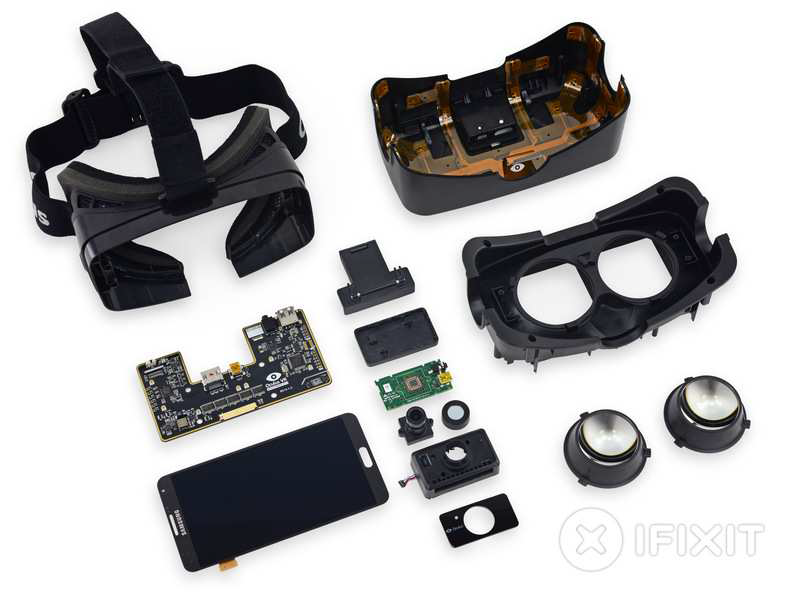
\includegraphics[width=0.65\textwidth]{figure/VisoreHW}
	\centering
	\caption{Lo schema di un sistema VR}
\end{figure}



\subsubsection{Software}
La componente software che permette la creazione di esperienze virtuali è gestita dal VWG citato in precedenza. Esso prende in input i dati dei sistemi di basso livello, che indicano cosa stia facendo l'utente nel mondo reale e li gestisce in modo che le componenti di \textit{rendering} possano creare una simulazione virtuale coerente e realistica.\\ La creazione dei mondi virtuali può essere gestita con diversi gradi di realismo, utilizzando mondi puramente sintetici, ovvero che esistono solamente nel contesto della simulazione 3D, oppure estremamente realistici che ricreano luoghi reali mappati in precedenza con l'utilizzo di camere digitali, e di tecniche di rielaborazione dell'immagine come lo \textit{SLAM}(\textit{Simultaneous Localiztion and Mapping}) e il \textit{texture mapping}. \\
\newline
La funzione base del software per un'applicazione VR rimane però il mantenimento della corrispondenza tra la posizione fisica e quella virtuale e del superamento di eventuali limiti qualora queste ultime non possano combaciare. Infatti nel caso in cui degli  ostacoli fisici nel mondo reale non fossero replicabili nel mondo virtuale, o più probabilmente il contrario, lo sviluppatore deve gestire questa incompatibilità. Per fare ciò si può ampliare il mondo virtuale se l'utente non è limitato in uno spazio nel mondo fisico, considerando però che al crescere della libertà di movimento concessa ad una persona durante l'esperienza crescono anche i relativi problemi di sicurezza dato il parziale oscuramento dei sensi. Un'altra soluzione che permette la navigazione di spazi virtuali infinitamente grandi è l'inserimento di un sistema \textit{locomotivo}, in cui l'indossatore si sposta nella simulazione stando in realtà fermo. Questo può essere implementato con l'ausilio di periferiche esterne. Purtroppo anche questa soluzione nasconde delle problematiche, poiché è facile indurre nell'utente effetti sgradevoli come il \textit{motion sickness}, ovvero la sensazione di nausea data dall'incoerente differenza tra la vista e il senso dell'equilibrio.\\
Una parte più complessa affidata al lato software è la gestione della fisica virtuale. Quest'ultima è di fondamentale importanza per rendere più credibile la realtà virtuale.\\
Difatti se nella simulazione facciamo cadere un oggetto, il nostro cervello si aspetta che cada proprio come nella realtà. Vengono quindi utilizzati degli algoritmi di \textit{rilevamento delle collisioni} che determinano se due o più oggetti si intersecano. Questo argomento raggiunge complessità così elevate quando si prendono in considerazione significative quantità di collisioni o gli effetti della propagazione di luce e suono virtuali, che sfocia in una disciplina a parte.
Nel caso di un'applicativo connesso alla rete, il mondo virtuale condiviso è mantenuto su un server che gestisce e aggiorna i movimenti o le varie interazioni degli utenti.\\
\begin{figure}[H]
	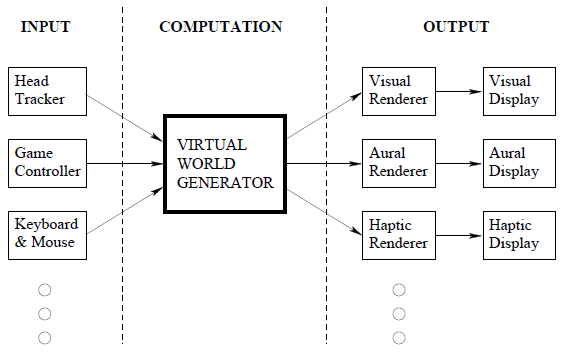
\includegraphics[width=0.65\textwidth]{figure/SoftwareBB}
	\centering
	\caption{le funzioni di uno VWG schematizzate}
\end{figure}

In conclusione, per lo sviluppo VR, si può partire dal SDR \textit{software development kit} di un visore che gestisca i driver e le componenti di basso livello come i sensori o le librerie grafiche, costruire da zero la fisica del mondo virtuale e implementare i requisiti dell'applicazione desiderata. Questo approccio consente di massimizzare le performance e amplia il controllo dello sviluppatore, ma è troppo complicato da gestire per applicazioni complesse. In questi casi si fa ricorso a VWG già pronti, lasciando in mano al creatore solo le componenti software ad alto livello. Alcuni esempi sono OpenSimulator, Vizard di WorldViz, Unreal Engine di Epic Games e Unity3D, che approfondiremo più avanti.

